\documentclass{beamer}
\usetheme{metropolis} % Use the metropolis theme




% Add tikz and pgfplots packages
\usepackage{tikz, pgfplots}
\usetikzlibrary{positioning}

% For clicking references
\usepackage{hyperref}

% For better horizontal lines
\usepackage{booktabs}

% For better referencing
\usepackage{cleveref}

\usepackage{graphicx}


\usepackage{amsmath}

\usepackage{wasysym}

% Define custom pastel colors
\definecolor{pastelRed}{RGB}{255, 105, 97}   % A soft pastel red
\definecolor{pastelBlue}{RGB}{119, 158, 203} % A muted pastel blue
\definecolor{pastelYellow}{RGB}{255, 223, 0} % A gentle pastel yellow
\definecolor{lightGray}{RGB}{211, 211, 211}  % A light gray for subtitles and less emphasized text

% Apply the custom colors
\setbeamercolor{palette primary}{bg=black, fg=white}
\setbeamercolor{palette secondary}{bg=lightGray, fg=black}
\setbeamercolor{palette tertiary}{bg=black, fg=white}
\setbeamercolor{titlelike}{parent=palette primary, fg=black}
\setbeamercolor{subtitle}{fg=lightGray}
\setbeamercolor{structure}{fg=black} % For itemize, enumerate, etc

% Change color of normal text
\setbeamercolor{normal text}{fg=black, bg=white}

% Set the color of the table of contents
\setbeamercolor{section in toc}{fg=black} % Section titles in TOC
\setbeamercolor{subsection in toc}{fg=black} % Subsection titles in TOC

% Set block colors
\setbeamercolor{block title}{use=structure,fg=white,bg=pastelRed}
\setbeamercolor{block body}{fg=black,bg=white}



% Title Page Info
\title{String Matching}
\subtitle{Spørgsmål 8 fra Exam Questions}
\author{Kevin Vinther}
\date{\today}

\begin{document}

% Title Page
\begin{frame}
  \titlepage
\end{frame}

% Table of Contents
\begin{frame}[allowframebreaks]
  \frametitle{Table of Contents}
  \tableofcontents
\end{frame}

\section{String Matching}
\label{sec:stringmatch}

\begin{frame}[allowframebreaks]
  \frametitle{String Matching}
  \begin{itemize}
  \item String Matching er, simpelt, et problem hvor vi er givet en tekst, og vil finde alle forekomster af en streng i teksten. Formelt:
  \item Vi antager at teksten er en array $T[1..n]$ af længde $n$ og at strengen vi leder efter er en array $P[1..m]$ hvor $m \leq n$. 
  \item Endvidere antager vi at elementer af $P$ og $T$ er karakterer fra alfabetet $\Sigma$. (husk til(bage til) formelle sprog.)
  \item Arraysne $P$ og $T$ kaldes ofte(st) strenge af karakterer. 
  \item Vi siger at et ``mønster'' (den streng vi leder efter) $P$ forekommer med \textit{shift} $s$ i teksten $T$. 
  \item (Eller, ækvivalent, at mønsteret $P$ begynder at forekomme i position $s+1$ i tekst $T$) 
  \item Dette gælder så længe at $0 \leq s \leq n - m $ og $T[s+1 .. s+m] = P[1..m]$ (altså, hvis $T[s+j] = P[j]$, for $1 \leq j \leq m$)
  \end{itemize}

 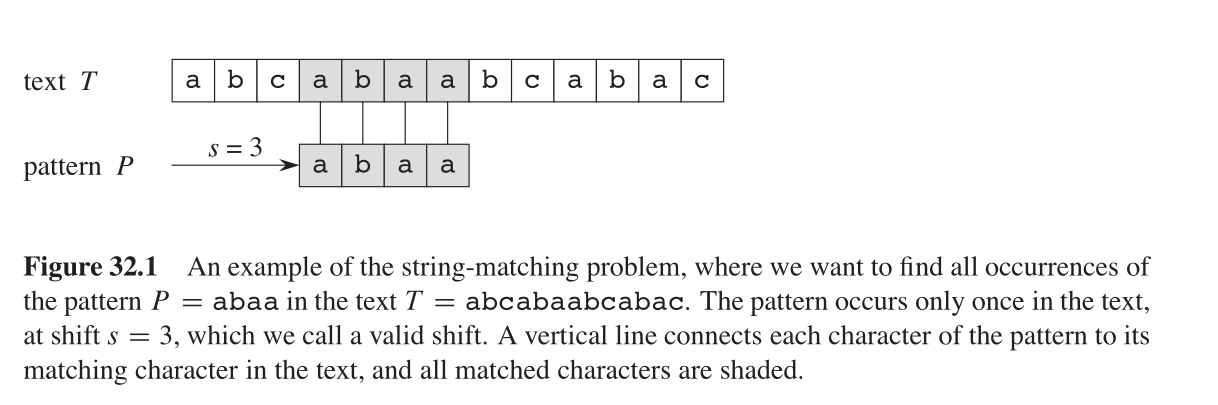
\includegraphics[width=350pt]{main--string-matching-4d75.png} 

 \begin{itemize}
 \item Hvis mønsteret $P$ forekommer med shift $s$ i $T$, kalder vi $s$ et \textbf{valid shift}, og ellers et \textbf{invalid shift}.
 \item String matching problemet er problemet om at finde \textbf{alle} valide shifts givet et mønster $P$ der forekommer i tekst $T$.
 \end{itemize}
\end{frame}

\begin{frame}
  \frametitle{Oversigt over string-matching algoritmer}
  
  \begin{table}[]
\centering
\begin{tabular}{lll}
\toprule
\textbf{Algorithm}          & \textbf{Preprocessing Time} & \textbf{Matching Time} \\
\midrule
\textit{Naive}              & $0$                         & $O((n-m+1)m)$          \\
\textit{Rabin-Karp}         & $\Theta (m)$                & $O((n-m+1)m)$          \\
\textit{Finite Automaton}   & $O(m |\Sigma |)$            & $\Theta (n) $          \\
\textit{Knuth-Morris-Pratt} & $\Theta (m)$                & $\Theta (n)$           \\
\bottomrule
\end{tabular}
\end{table}
\end{frame}

\begin{frame}[allowframebreaks]
  \frametitle{Preprocessing}
 \begin{itemize}
 \item Alle algoritmer med undtagelse af den naive laver noget preprocessing baseret på et mønster og finder så alle valide shifts. 
 \item At finde de valide shifts kalder vi ``matching''
 \item Rabin Karp har en langt bedre average-case på trods af at dens worst case er det samme som naiv.
 \end{itemize} 
\end{frame}

\begin{frame}[allowframebreaks]
  \frametitle{Terminologi}
 \begin{itemize}
 \item Vi betegner sættet af alle endelige strenge formet af alfabetet $\Sigma$ som værende $\Sigma^*$
 \item Bemærk at $\varepsilon$ (den tomme streng) også er en del af $\Sigma^{*}$.
 \item Længden af en streng, $x$ bliver betegnet som $|x|$
 \item Concatenation bliver betegnet som $xy$ og har længden $|x| + |y|$. Der er, simpelt, karaktererne i $x$ efterfulgt af karaktererne i $y$.
   \item Vi siger at $\omega$ er et præfix af en streng $x$, betegner $\omega \sqsubset x$, hvis $x = \omega y, y \in \Sigma^{*}$. 
   \item Bemærk at hvis $\omega \sqsubset x$, så $|w| \leq |x|$. 
   \item Endvidere siger vi at $\omega$ er et suffix af en streng $x$, betegnet $x \sqsupset x$, hvis $x = y \omega$ for en $y \in \Sigma^{*}$. 
   \item Som med et præcis, hvis $w \sqsupset x$ så $|\omega| \leq |x|$.
   \item Bemærk også at $\sqsubset $ og $\sqsupset$ er transitive relationer. 
 \end{itemize} 
 \begin{lemma}[31.1 (Overlapping-suffic lemma)]
Suppose that $x, y, $ and $z$ are strings such that $x \sqsupset z$ and $y \sqsupset z$. If $|x| \leq |y|$, then $x \sqsupset y$. If $|x| \geq |y|$, then $y \sqsupset x$. If $|x| = |y|$, then $x = y$.
\end{lemma}
\begin{itemize}
\item Vi bruger et grafisk bevis:
\end{itemize}
\vspace{1cm}
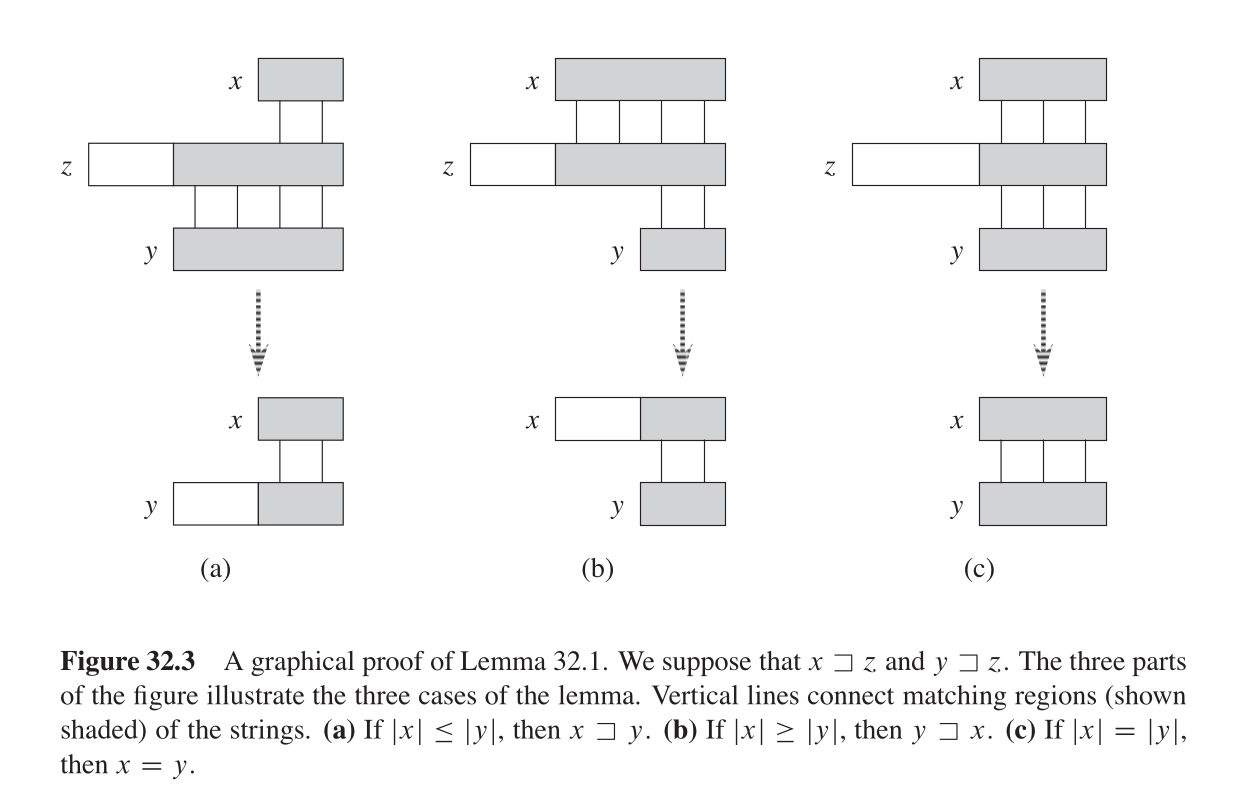
\includegraphics[width=330pt]{main--string-matching-c1c3.png}
\vspace{1cm}

\end{frame}

\begin{frame}[allowframebreaks]
  \frametitle{Terminologi}
  
\begin{itemize}
\item For lethed af notation, betegner vi en $k$-karakters præfix $P[1..k]$ af møsteret $P[1..m]$ af $P_{k}$. Dermed $P_{0} = \varepsilon$, $P_{m} = P = P[1..M]$ (så længe man går ud fra at længden af $P$ er $m$.)
\item Ved brug af denne notation kan vi sige at string-matching problemet er det hvor vi skal finde alle shifts $s$ i rangen $0 \leq s \leq n -m$ således at $P \sqsupset T_{s+m}$.
\item I den pseudokode vi kommer til at bruge, tillader vi to strenge på samme længde til at blive sammenlignet som en primitiv operation (som +, - etc).
\item Hvis strengene bliver sammenlignet venstre til højre og sammenlignningen stopper når et mismatch er fundet, kan vi assume at tiden taget er en lineær funktion af antallet af sammenlignet karakterer fundet. 
\item Så, for at være præcis, testen \texttt{x == y} er antaget at tage tiden $\Theta (t+1)$, hvor $t$ er længden af den længste streng $z$, således at $z \sqsubset x$, og $z \sqsubset y$. (Vi skriver $\Theta (t+1)$ i stedet for $\Theta(t)$ for at kunne tage den case hvor $t = 0$)
\end{itemize}
\end{frame}

\section{The Naive String-Matching Algorithm}
\label{sec:label}


\begin{frame}
  \frametitle{Den Naive String-Matching Algorithme}
  \begin{itemize}
  \item Den naive (brute-force) string-matching algoritme finder alle valide shifts ved brug at et loop. 
  \item Loopet tjekker condition $P[1..m] = T[s+1 .. s+m]$ for hver linje af de $n-m+1$ mulige værdier a $s$. 
  \end{itemize}
  
  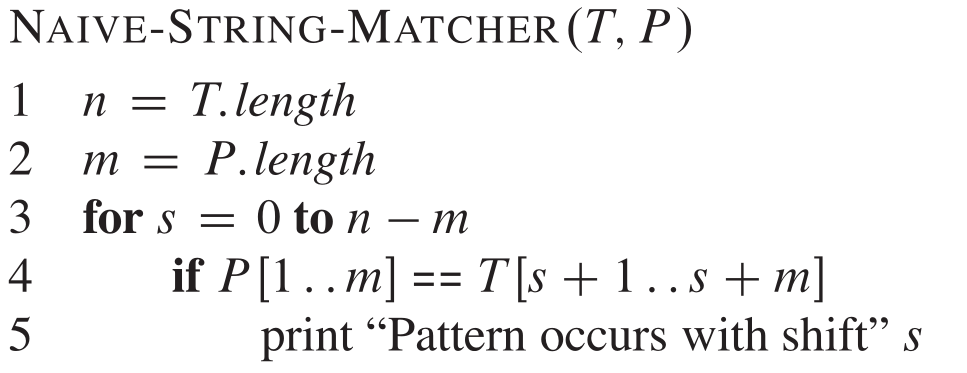
\includegraphics[width=300pt]{main--the-naive-string-matching-algorithm-3b93.png}
\end{frame}

\begin{frame}[allowframebreaks]
  \frametitle{Naive Approach}
  \begin{itemize}
  \item Køretiden på denne algoritme er $O((n-m+1)m)$ hvilket er ret lort. 
  \item Det kan blive $\Theta (n^{2})$ hvis vi har en streng $a^{n}$ og et mønster $a^{m}$, og $m = \lfloor n / 2 \rfloor$. 
  \item Til gengæld ingen preprocessing!
  \end{itemize}
\end{frame}


\begin{frame}[allowframebreaks]
  \frametitle{Rabin-Karp}
  \begin{itemize}
  \item Det var da godt nok lort, hva? 
  \item Tid til Rabin-Karp som (måske nok) er bedre!
  \item Preprocessing tid: $\Theta (m)$
  \item Køretid worst-case: $\Theta ((n-m+1)m)$.
  \item Dog er køretiden bedre baseret på nogle assumptions. 
  \item Antag at $\Sigma = \{0, 1, 2, \ldots, 9\}$.
  \item Så kan vi se en streng af $k$ konsekutive karakterer som et længde-$k$ decimaltal.
  \item F.eks. kan strengen $31415$ ses som decimaltallet $31,415$. 
  \item Givet et mønster $P[1..m]$, lad $p$ betegne dens korresponderende decimalværdi. 
  \item I en lignende manér, givet en tekst $T[1..n]$, lad $t_{s}$ betegne decimlaværdien af længde-$m$ substrengen $T[s+1..s+m]$, for $s = 0, 1, \ldots, n -m$. 
  \item Hvis $t_{s} = p$ så er $T[s+1..s+m] = P[1..m]$.
  \item Dermed er $s$ et \textbf{valid shift} iff $t_{s} = p$. 
  \item Hvis vi kan udregne $p$ i $\Theta(m)$ tid, og alle $t_{s}$ værdier i alt på en tid af $\Theta (n-m+1)$ tid, kan vi vælge alle valide shifts $s$ i tiden $\Theta(m) + \Theta(n-m+1) = \Theta(n)$ ved at sammenligne $p$ med hver af de $t_{s}$ værdier. 
  \item Vi kan udregne $p$ i tid $\Theta(m)$ ved brug af \textbf{Horner's Regel:}
  \item $p = P[m] + 10 (P[m-1]+ 10 (P[m-2] + \cdots + 10(P[2] + 10P[1]) \cdots ) ) $
  \item For at udregne de resterende værdier $t_{1}, t_{2}, \ldots, t_{n-m}$ i $\Theta(n-m)$, observerer vi at vi kan udregne $t_{s+1}$ fra $t_{s}$ i konstant tid, siden: 
  \item $t_{s+1} = 10(t_{s}-10^{m-1}T[s+1]) + T[s+m+1]$
  \end{itemize}
  
\end{frame}


\end{document}